% !TEX root = rob1.tex
\chapter{Regelung von Robotersystemen}
\textbf{Laufende Beobachtung bei der mit den gewonnenen Informationen die Stellgröße derart
verändersot wird, dass trotz Störgrößeneinwirkung die Ausgangsgröße an den gewünschten Verlauf
(Sollverlauf) angeglichen wird.}

\section{Regelkreis}
\begin{figure}[!h]
    \centering
    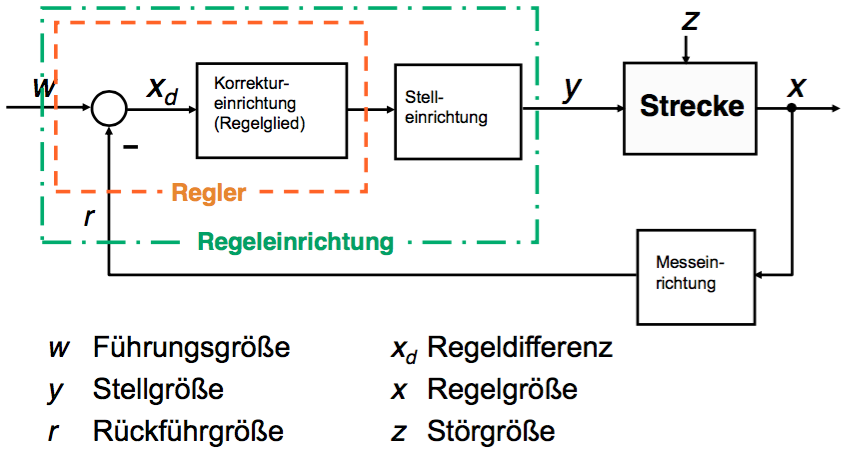
\includegraphics [scale=0.5]{regelkreis}
    \caption{Struktur eines Regelkreises}
\end{figure}

\mparagraph{Wirkungsweise}
\textbf{z} wird größer $\Rightarrow$ \textbf{x} wird gesenkt $\Rightarrow$ \textbf{r} wird abgesenkt
$\Rightarrow$ \textbf{$x_d$} wird angehoben $\Rightarrow$ \textbf{y} wird angehoben $\Rightarrow$
\textbf{x} wird angehoben mit der Tendenz den Sollwert \textbf{$x_s$} wieder anzunehmen. \\
Die Störgröße wird ausgeregelt.

\section{Grundlagen}
\subsection{Laplace Transformation}
\begin{compactitem}
    \item Rechenvereinfachung: Differential und Integralausdrücke werden zu algebraischen Ausdrücken.
    \item Gleichungslösung im Frequenzbereich statt Zeitbereich
    \item Integral muss konvergieren $\rightarrow$ lineare $f(t)$
\end{compactitem}
\begin{displaymath}
     L[f(t)] = f(s) = \int_0^\infty f(t)e^{-st}dt, s := \sigma + j\omega \text{ in } C \text{  } f(t)
      = 0, t < 0
\end{displaymath}

\begin{compactitem}
    \item \textbf{Linearitätssatz}: $L[\alpha f_i(t) + \beta f_2(t)] = \alpha f_1(s) + \beta f_2(s)$
    \item \textbf{Faltungssatz}: $L[f_1(t) * f_2(t)] = f_1(s) * f_2(s)$
    \item \textbf{Grenzwertsatz}: $f_1(t = 0) = \lim_{s \rightarrow \infty} s * f(s)$
    \item \textbf{Differentiationssatz}: $L[\frac{d}{dt}f(t)] = sF(s)$
    \item \textbf{Integrationssatz}: $L[\int f(t)dt] = \frac{1}{s}F(s)$

\end{compactitem}
\subsection{Übertragungsglieder}
\begin{compactitem}
    \item \textbf{P-Glied}: $y(t) = K * u(t)$
    \item \textbf{I-Glied}: $y(t) = K * \int_0^t u(\tau)d\tau$
    \item \textbf{D-Glied}: $y(t) = K * \dot{u}(t)$
    \item \textbf{T$_t$-Glied}: $y(t) = K * u(t-T_t)$
    \item \textbf{S-Glied}: $y(t) = K * \pm u_1(t) \pm u_2(t)$
    \item \textbf{KL-Glied}: $y(t) = K * F(u(t))$
    \item \textbf{M-Glied}: $y(t) = K * u_1(t)u_2(t)$
\end{compactitem}

\section{Reglertypen}
\subsection{PID Regler (und Unterklassen)}
\textbf{Sehr verbreitet, da für nahezu alle Prozesstypen geeignet, robust und mit geringem Aufwand
realisierbar} \\
P: güngstiges Regelverhalten, I: stationäre Genauigkeit, D: schnelle Ausregelung
\begin{align}
    u(t) = K_p (e(t) + \frac{1}{T_N}\int_o^t e(\tau)d\tau)+ T_V \frac{d}{dt}e(t))
\end{align}
mit Nachstellzeit $T_N$ und Vorhaltzeit $T_V$.

\mparagraph{Laplacetransformation}
\begin{align}
    u(t) &= K_Pe(t) + K_I \int e(t)dt + K_D \frac{d}{dt}e(t) \Leftrightarrow \\
    \Leftrightarrow u(s) &= K_Pe(s) + K_I \frac{1}{s}e(s) + K_Dse(s) \\
    \leftrightarrow \frac{u(s)}{e(s)} &= G(s) = K_P + K_I \frac{1}{s}+K_Ds \\
    \frac{\text{Ausgang}}{\text{Eingang}} &= \text{Übertragungsfunktion}
\end{align}
\subsection{Kennlinien- bzw. Kennlinienfeldregler}
\textbf{nihctlineare Übertragungsglieder}\\
z.B Zweipunktregler (Temperatur-Regelung)
\newpage
\subsection{Zustandsregler}
\textbf{Verbessertes Regelverhalten, da nicht nur die Regelabweichung, sondern im Idealfall alle
Zustandsgrößen der Regelstrecke zur Verfügung gestellt werden.} \\
regelungstechnische Behandlung von Mehrgrößensystemen, nichtlinearen und zeitvariablen
Übertragungssystemen.

\begin{figure}[!h]
    \centering
    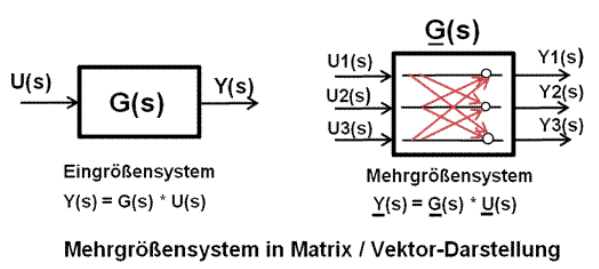
\includegraphics [scale=0.5]{mehrgroesse}
\end{figure}

\subsection{Kaskadenregelung}
\textbf{Unabhängige lineare Einzelregelkreis der einzelnen Gelenke}\\
Manipulator = Mehrgrößensystem

\begin{figure}[!h]
    \centering
    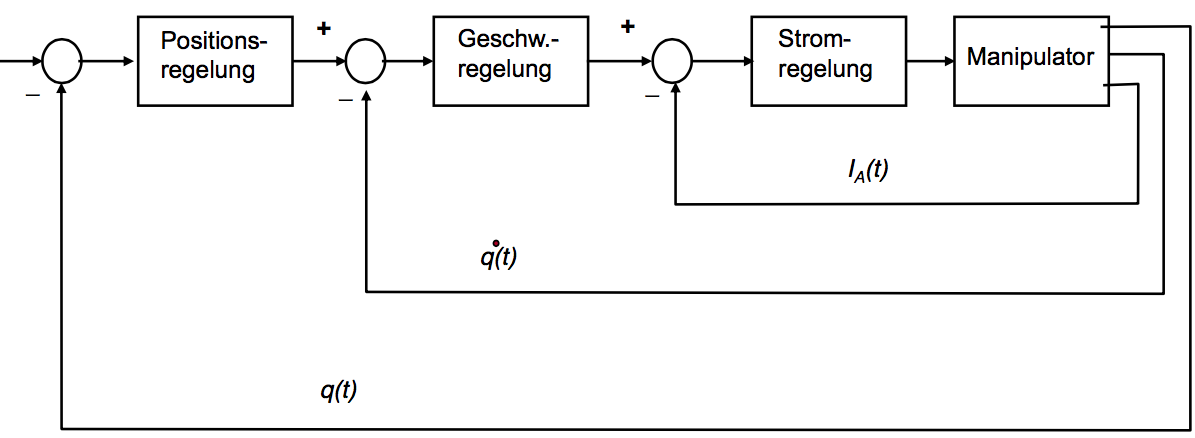
\includegraphics [scale=0.3]{kaskade}
\end{figure}

\subsection{Adaptive Regelung}
\textbf{Lageabhängige und somit zeitveränderliche Systemteile werden als Parameterschwankungen
aufgefasst}
\begin{figure}[!h]
    \centering
    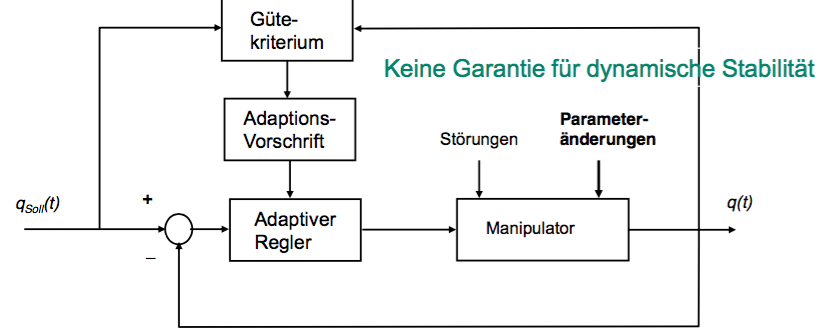
\includegraphics [scale=0.3]{adaptiv}
\end{figure}

\section{Regelungskonzepte für Manipulatoren}
\textbf{Regelung von Manipulatoren beschreibt nicht nur Positionsregelung, sondern auch die
Einbeziehung weiterer Umwelteinflüsste} (Massenträgheit des Manipulators, Gravitations-, Zentrifugal-,
Coriolis und Reibungskräfte/Momente auf die Gelenke)
\subsection{Exakte Systemmodellierung}
setzt a priori die exakte Kenntnis des Dynamikmodells und er Umgebung des Roboters voraus.
\subsection{Kraft-/Positionsregelung}
Position und Kräfte sind eng miteinander verknüpft. Steht Roboter in Kontakt mit Umgebung so bedeutet
Positionsänderung auch Kraftänderung und vice versa.

\mparagraph{Hybride Kraft-/Positionsregelung}
Wahlweise zwischen reiner Kraft und reiner Positionsregelung gewählt für jede kartesische Bewegungsrichtung
des Arms.
\mparagraph{Impedanz Regelung}
Regelt die dynamische Beziehung zwischen Kraft und Positions im Kontaktfall. \\
Idee: Interaktion Roboter-Umwelt verhält sich wie Feder-Dämpfer-Masse-System.
\begin{align}
     f(t) &= d * x(t)b * \dot{x}(t) + m * \ddot{x}(t)\\
     &\Rightarrow \text{Lapace Transformation} \Rightarrow \\
     F(s) &= (d + b+ s+ m *s ^2) * X(s)
\end{align}
Impedanz kann über Steifheit d, Dämpfung b und Trägheit m beeinflusst werden.
